\chapter{External toolboxes}
\thispagestyle{fancy}



\section{User contributed software}
Besides the algorithms that come with the \MATLAB{} program, there is a wealth of user-contributed programs available on the Internet. A good place to look for such programs, is the `File Exchange' on the Mathworks website \url{http://www.mathworks.com/matlabcentral/fileexchange/?sort=downloads}.

\begin{action}
Take 20 minutes to browse through the contents of the File Exchange website. On the left side of the website, there is an item `Files by Category' that you may want to use to limit the search to the `Earth Sciences' domain. 
\end{action}
As you can see, there are many programs available that you can use for free. In this chapter we will use the GoogleEarth Toolbox for \MATLAB{}\index{GoogleEarth Toolbox for MATLAB@GoogleEarth Toolbox for \MATLAB{}}: \url{http://www.mathworks.com/matlabcentral/fileexchange/12954-google-earth-toolbox}. You have a copy of the GoogleEarth Toolbox, located in the folder `pim\_files\textbackslash{}'. In this chapter, you will learn to use the functions in this toolbox.

\project{Google Earth Toolbox}
\label{pr:googleearth}

\section{Installing GoogleEarth}
\begin{action}
Open Windows Explorer and navigate to the folder `pim\_files\textbackslash{}ch13\_toolboxes'. There should be a file `GoogleEarthPerUserSetup.exe'. Click to install the GoogleEarth Viewer.\index{GoogleEarth Viewer}
\end{action}

\section{Setting up the GoogleEarth application}
To avoid problems with displaying and interpreting your GoogleEarth files, it's necessary to have your copy of GoogleEarth set up according to the following specifications:
\begin{enumerate}
\item Click \guitext{Tools} in GoogleEarth's menu and choose \guitext{Options\ldots}. On the tab named \guitext{3D View} check that \guitext{Graphics Mode} is set to \guitext{OpenGL}\index{OpenGL}.
\item On the same tab, set the latitude/longitude format to \guitext{Decimal Degrees} under \guitext{Show Lat/Long}.
\item Also on this tab, set the units of elevation to \guitext{Meters, Kilometers} under \guitext{Show Elevation}.
\end{enumerate}



\section{KML}
The great flexibility of GoogleEarth stems from its use of XML\index{XML}\footnote{\url{http://en.wikipedia.org/wiki/XML}}-based text files, known as KML\index{KML}\index{Keyhole Markup Language}\footnote{\url{http://en.wikipedia.org/wiki/Keyhole_Markup_Language}}-files (you can recognize these files by their extension *.kml\index{*.kml}). Such a file typically contains a series of objects, such as polygons, lines and points. Each of these objects is represented within a KML-file by its KML-tags. For example, we may find a polygon object:
\begin{verbatim}
<Polygon>
...
</Polygon>
\end{verbatim}
Or a line object:
\begin{verbatim}
<LinearRing>
...
</LinearRing>
\end{verbatim}
\vspace{1em}

\noindent Properties such as line width, coordinates, and polygon color may be specified using additional tags. A line may thus be assigned a line style as follows:
\begin{verbatim}
<LineStyle>
   <color>ffffffff</color>
   <width>1.00</width>
</LineStyle>
\end{verbatim}
Which represents a fully opaque, white line of width 1.

\subsection{Automated writing of KML}
Of course, writing KML-tags by manually typing them in a text editor is not practical when working with data containing more than just a few objects. Fortunately though, the task of writing these files can be fully automated using the GoogleEarth Toolbox.

The GoogleEarth Toolbox generates plain ASCII text files. The text contained within these files is formatted according to the Keyhole Markup Language (KML) specification, which allows for a hierarchical organization of the objects and properties contained within the file. KML files can be opened in the GoogleEarth Viewer.

The GoogleEarth Toolbox implements a number of low-level functions for displaying point, line and polygon objects within GoogleEarth. In addition to that, higher-level methods include functions to visualize 2D rasterized data, create contour maps, surface and quiver plots, image overlays (in GIS usually referred to as \textit{draping}), and a few others.

\section{Structure of the GoogleEarth Toolbox}
The core of the toolbox is formed by a set of about 20 \MATLAB{} functions (*.m files) located in the toolbox root folder (`googleearth/'). The majority of these functions generate character arrays in concordance with the KML standard. For each of the m-files, a help file has been included which can be viewed from within the \MATLAB{} help browser. The help files are located in `googleearth/html'. In addition to the help files, demonstrations have been included (`googleearth/demo'). Many of these demos write their output to a separate folder (`googleearth/kml') in order to avoid contaminating directories with files that do not belong there. Folder `googleearth/data' contains additional files such as icon images and Collada models. Folder 'googleearth/doc' contains files pertaining to the printable documentation. Finally, a folder 'googleearth/tmp' has been included, which is used by some functions to write temporary data to. The contents of this folder are automatically emptied by some functions, therefore you should not save important data in it. In fact, it's best if you don't save any file anywhere under `googleearth/'.


\section{Adding the toolbox to the path}
When you use a function name in your scripts or at the prompt, \MATLAB{} starts searching a predefined list (i.e. the `path') of directories where \MATLAB{} functions are stored. 
\begin{action}
At the prompt, type
\prompt{path}\index{path@\textt{path}}
\end{action}
The default list of directories should now be displayed in the command window. In order to use the functions from the GoogleEarth Toolbox, you need to add the toolbox' top-level directory to the path:
\prompt{addpath(\squote{D:\textbackslash{}matlab\textbackslash{}googleearth})}\index{addpath@\texttt{addpath}}
\noindent This will add the indicated directory to the \MATLAB{} search path (see {\tt doc path}). The above command is equivalent to using \guitext{Set Path\ldots} from the \guitext{File} menu of the \MATLAB{} Graphical User Interface. 

\begin{action}
Now type
\prompt{googleearth -docinstall}\index{googleearth@\texttt{googleearth}}
to initialize some files that are needed to use the documentation.
\end{action}
\vspace{1em}
\noindent After adding the toolbox location to the \MATLAB{} path, its functions may be called either from the command window or in scripts. Additionally, the toolbox documentation is accessible through the usual {\tt doc} command. Typing
\prompt{doc googleearth}
\noindent and following the hyperlink will take you to an index page where all functions are listed, along with a short description of their intended usage. As an alternative to using the {\tt doc} command, the documentation may also be accessed by selecting the GoogleEarth item which is now located under \MATLAB{}'s Start button \ding{217} Toolboxes (see Figure~\ref{fig:googleearth-help-menu}). In the documentation files, you can find information on what a particular function does, what variables to pass it, the function's options, links to other functions that perform related tasks, and an example of how the function can be used.


\begin{figure}[!htb]
  \centering
    \fbox{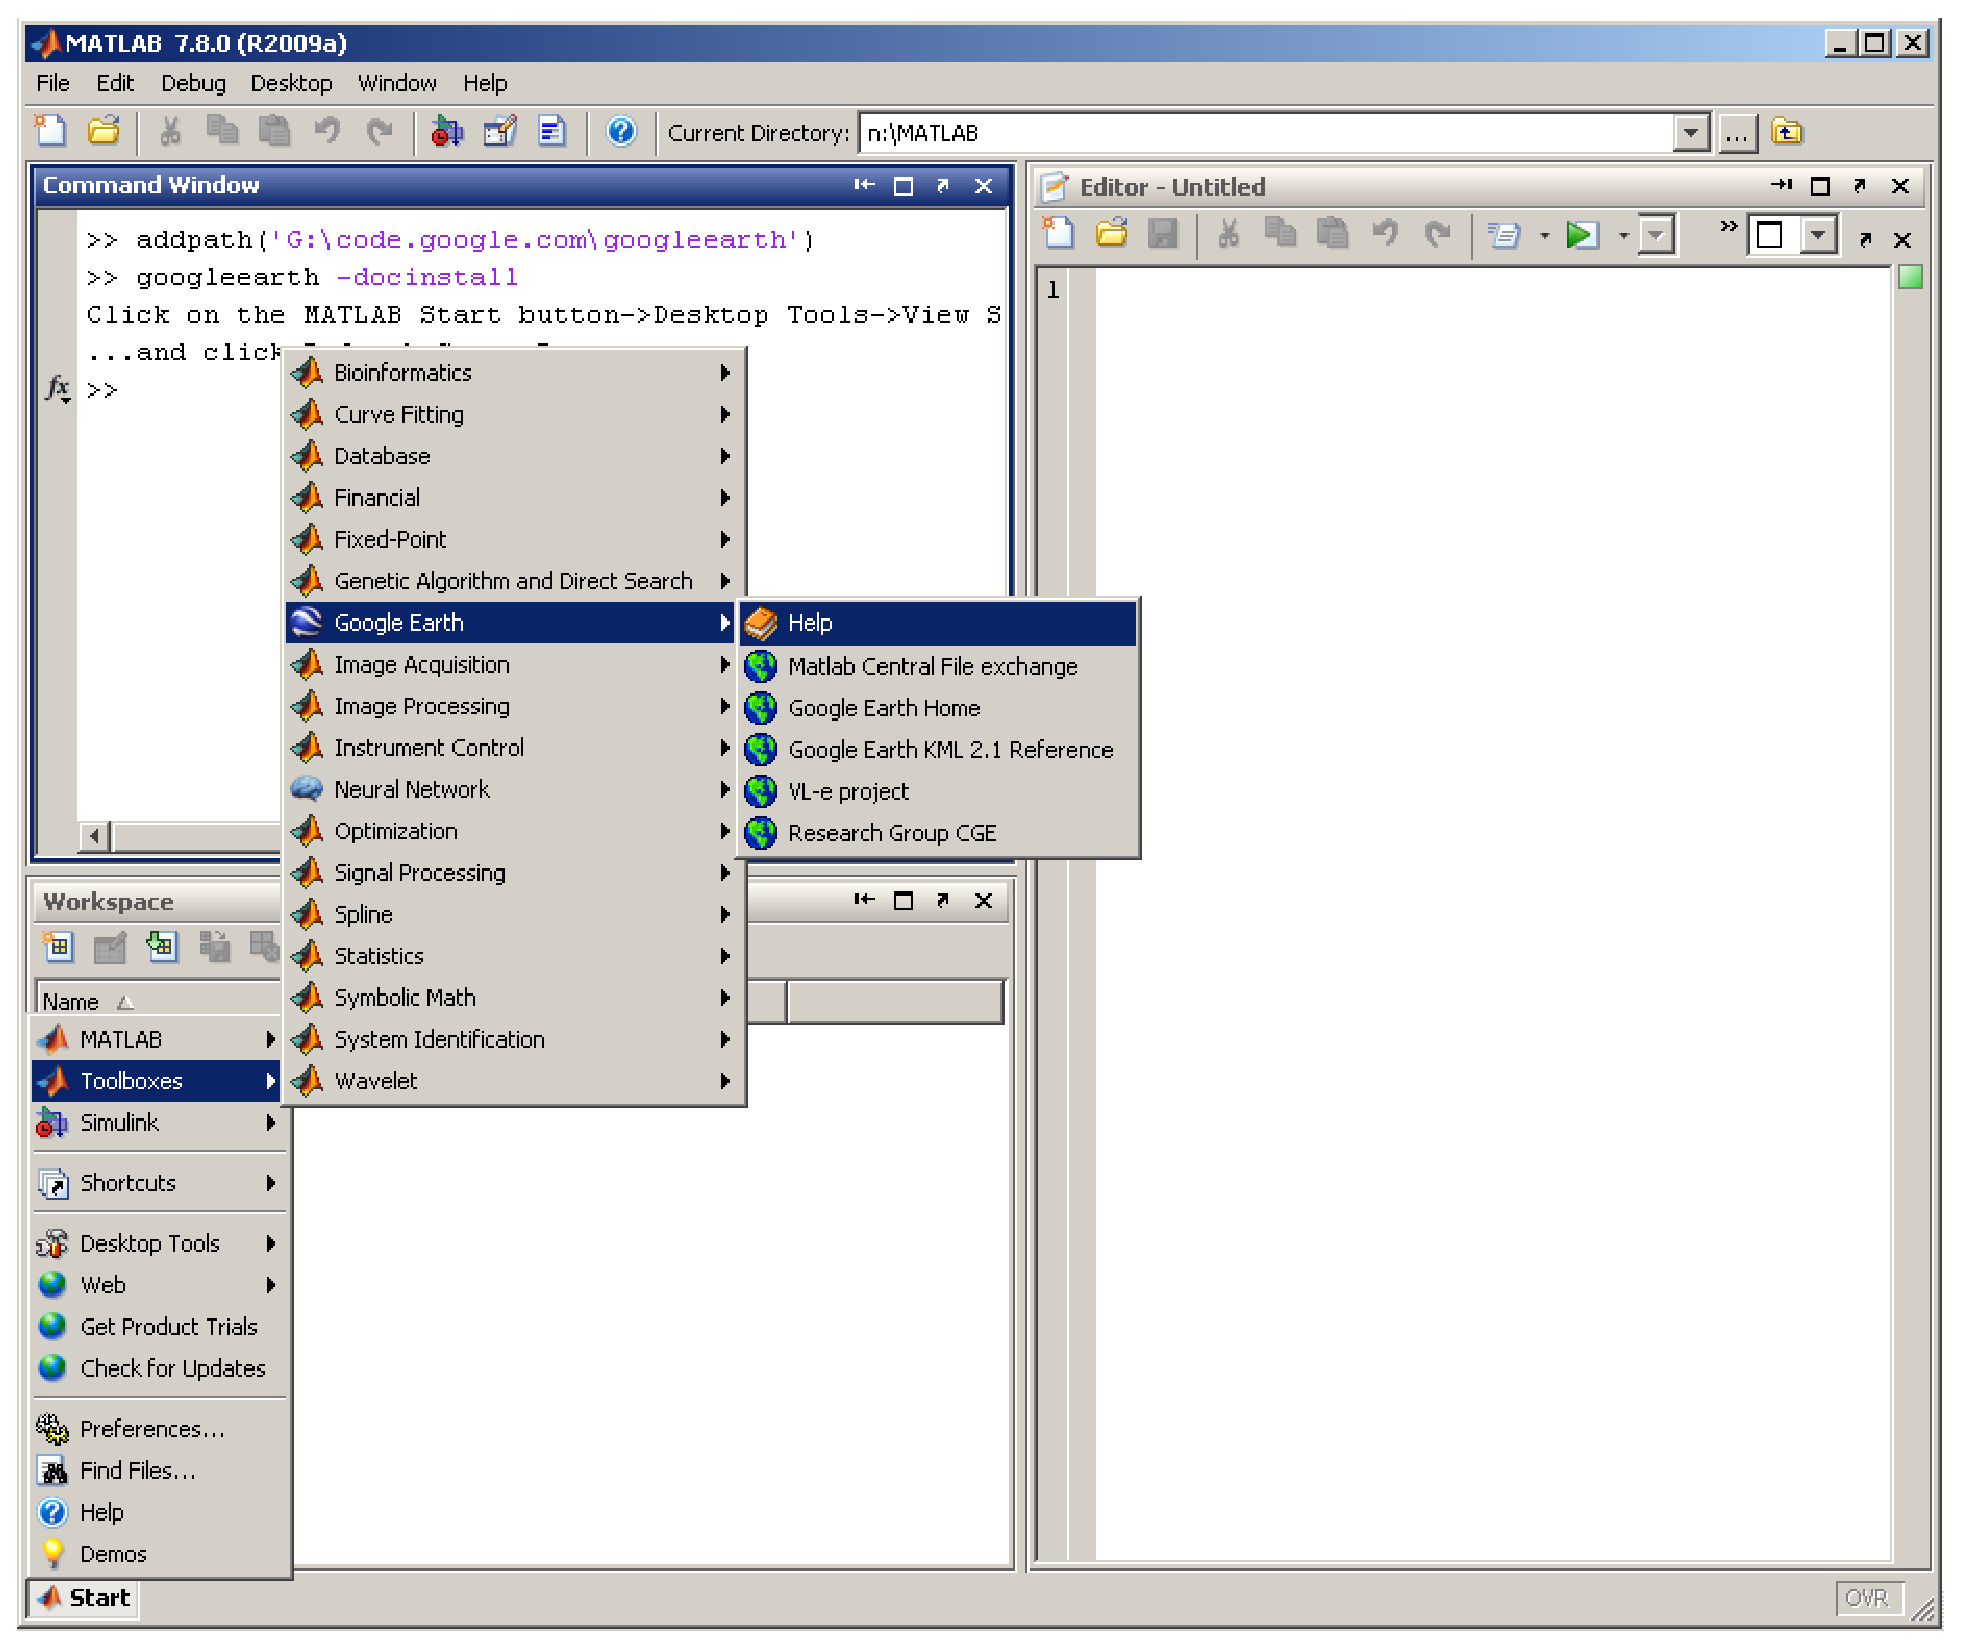
\includegraphics[width=1.0\textwidth]{./../eps/googleearth-help-menu.eps}}
  \caption{Accessing the GoogleEarth Toolbox documentation.}\label{fig:googleearth-help-menu}
\end{figure}







\section{Point features}
\begin{action}
In the GoogleEarth Viewer, go to a location of your choice and write down its latitude and longitude. 
\end{action}

\begin{action}
Navigate to the documentation on {\tt ge\_point}\index{ge\_point@\texttt{ge\_point}} or enter the command below at the prompt:
\prompt{doc ge\_point}
This should invoke the documentation about {\tt ge\_point}. Read through it carefully.
\end{action}

\begin{action}
Begin a new m-file called `\starred{name}\_point.m'. Let the script generate a character array called {\tt kmlStr}, which contains the location of your choice in KML format.
\end{action}
You should now have a character array with KML-formatted text. However, to be able to see your point in the GoogleEarth Viewer, we need to write the character array to a *.kml file.
\begin{action}
Consult the documentation on {\tt ge\_output}\index{ge\_output@\texttt{ge\_output}}, and use it to save your KML-formatted text to a *.kml file. 
\end{action}

\begin{action}
Open your *.kml file in the GoogleEarth Viewer and verify that it shows a point at the location of your choice.
\end{action}

\begin{action}
By default, the point is labeled with the full filename of its *.kml file when opened in the GoogleEarth Viewer (see left-hand pane \guitext{Places}). It's often useful to assign a different name to the object when viewed in GoogleEarth using {\tt ge\_output}'s parameter {\tt \squote{name}}. Change how your point is displayed in the \guitext{Places} pane in the GoogleEarth Viewer.
\end{action}

\begin{action}
Instead of the default placemarker icon, use this {\tt \squote{iconURL}}\index{`iconURL@\texttt{\squote{iconURL}}} (or any other icon of your choice): \url{http://maps.google.com/mapfiles/kml/pal3/icon35.png}.
\end{action}


\section{Line features}
Lesser black backed gulls (\textit{Larus fuscus}) are sea birds that spend spring and summer in The Netherlands but, like some of its human inhabitants, spend their winters in Southern Europe. While migration patterns of sea birds have been monitored before, until now it was not possible to get the detailed information about their movements needed to gain insight into their foraging behavior. Therefore, the University of Amsterdam developed a new flexible tracking system that enables detailed monitoring of the bird's movement. These so-called `GPS-loggers' consist of a tiny GPS system combined with a miniature recording device and transceiver, powered with a solar panel. They weigh only 18 grams, allowing birds to carry them on their backs without being restricted in their movements (see Figure~\ref{fig:lesser-black-backed-gull}). Once attached to the birds, the devices record their position, wing beat frequency, temperature and air pressure during their local and migratory movements with great detail.
In this section, you will use the GoogleEarth Toolbox to visualize the migratory route that gull~\#41745 has taken.
\begin{figure}[!htbp]
  \centering
    \fbox{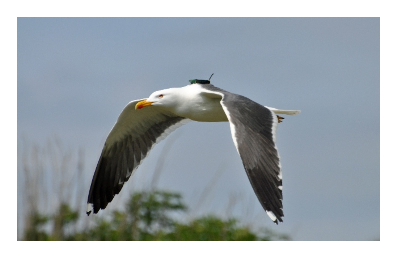
\includegraphics[width=1.0\textwidth]{./../eps/lesser-black-backed-gull.eps}}
  \caption{Lesser black-backed gull (\textit{Larus fuscus}) equipped with a GPS logger (Photo: Cees Camphuysen, NIOZ).}\label{fig:lesser-black-backed-gull}
\end{figure}

\begin{action}
Start a new script `\starred{name}\_seagull.m'. 
\end{action}
\begin{action}
Use {\tt textread} to load the seagull data from the file `pim\_files\textbackslash{}ch13\_toolboxes\textbackslash{}larus-fuscus.txt'. If you are not successful doing this but there's no one around to help you, use {\tt load(\squote{larus-fuscus-cheat.mat})} to read from a binary file, so that you won't waste too much time. (But don't forget to ask about {\tt textread} later).
\end{action}
\begin{action}
Consult the documentation on the use of {\tt ge\_plot}\index{ge\_plot@\texttt{ge\_plot}}, and use it to visualize the bird's track. Adapt the script so that it produces a fully opaque, red line of width 1.5. If you do this correctly, the data should be displayed as in Figure~\ref{fig:larus-fuscus}.
\end{action}
\begin{figure}[!htbp]
  \centering
    \fbox{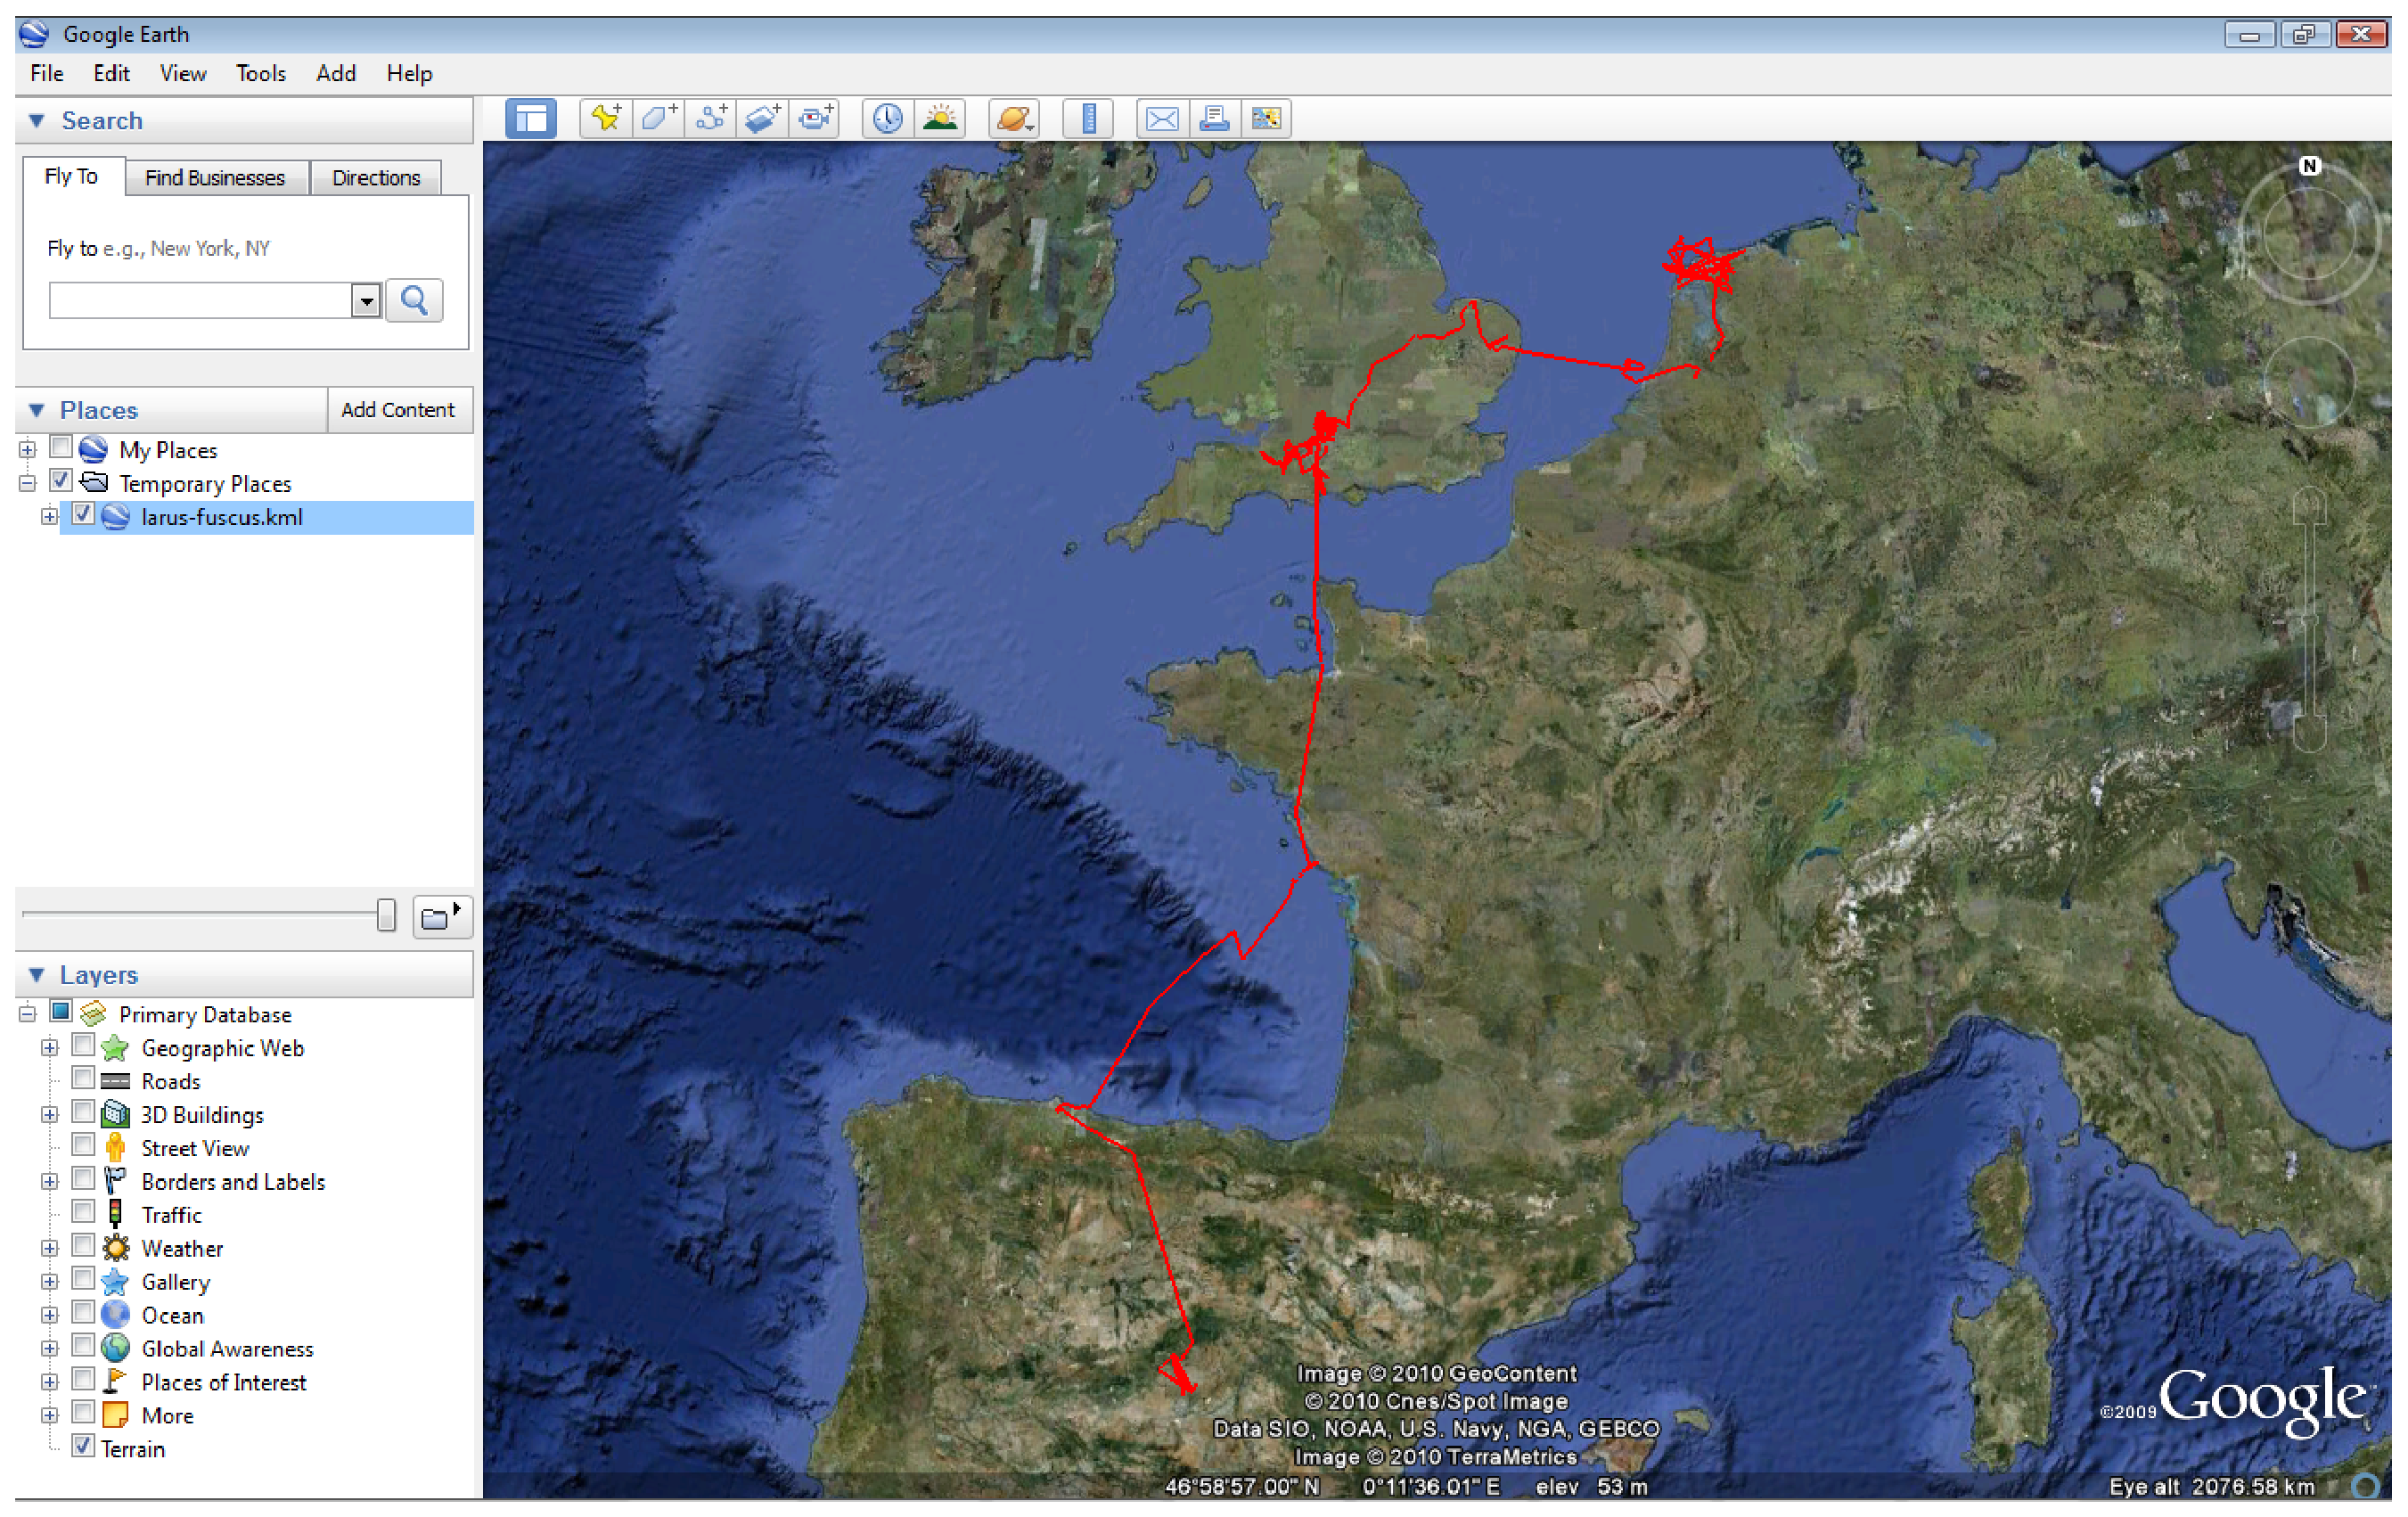
\includegraphics[width=1.0\textwidth]{./../eps/larus-fuscus.eps}}
  \caption{Bird track of seagull \#41745.}\label{fig:larus-fuscus}
\end{figure}

\begin{action}
Alter your script in such a way that it displays a point for each location where a measurement was taken. For this, you need to iterate over the locations, generate a {\tt ge\_point}, and concatenate the result with the KML-text that you already had. You can use any icon that you like (but \url{http://maps.google.com/mapfiles/kml/pal2/icon26.png} is a good option, especially when used in combination with the {\tt \squote{iconScale}}\index{`iconScale@\texttt{\squote{iconScale}}} and {\tt \squote{iconColor}}\index{`iconColor@\texttt{\squote{iconColor}}} options). If you open your *.kml file in the GoogleEarth Viewer, you should see the red line of Figure~\ref{fig:larus-fuscus}, as well as many points.
\end{action}

\noindent So far, you have generated KML files that contain objects which are static, i.e. they do not change with time. However, sometimes you want to present your data in a dynamic way, somewhat like a movie. The KML specification allows for the inclusion of objects which are visible only during a particular time interval. To make this work, the object in question (such as a point or a line) needs to be assigned a start time and an end time, between which it will be visible. The start and stop times need to be passed as character arrays using the option {\tt \squote{timeSpanStart}}\index{`timeSpanStart'@\texttt{\squote{timeSpanStart}}} and {\tt \squote{timeSpanStop}}\index{`timeSpanStop'@\texttt{\squote{timeSpanStop}}}. The character array should be formatted according to the following layout: {\tt 2008-01-05T22:00:00Z} , or 10 PM on the 5$^{th}$ of January 2008.

\begin{action}
Alter your {\tt textread} call in such a way that, in addition to the latitude and longitude, the time information is now also loaded into the workspace as two separate variables {\tt startDateTime} and {\tt endDateTime}.
\end{action}

\begin{action}
Use a {\tt for}-loop to iterate over all measurements. For each measurement, generate a KML string using {\tt ge\_point} with the timespan options. Concatenate and write to a *.kml file as before. When opened in the GoogleEarth Viewer, you should see a line representing the entire migratory route of the gull, as well as a point representing its location at a particular time. When played back, the point should move along the migratory route.
\end{action}

\hintbox{When the objects in the GoogleEarth Viewer are dynamic (i.e. when they have time labels), the upper left part of the main window contains additional controls with buttons for playback of the KML objects.}

\vspace{-2em}

\section{Rasterized imagery}
In the domain of Earth Sciences and Biology, we often have data in the form of maps. In this section, you will use the GoogleEarth Toolbox to visualize a map of Zinc concentrations in the Meuse river valley near Stein, The Netherlands. An array with spatial predictions of Zinc has already been derived from point measurements by means of a geostatistical method (ordinary kriging). This data is available as `pim\_files\textbackslash{}ch13\_toolboxes\textbackslash{}ok-predictions-radius.mat'.

\begin{action}
Start a new script `\starred{name}\_zinc.m'. Let it load the kriging data\footnote{Data from: Rikken, M.~G.~J. and Van Rijn, R.~P.~G. (1993) \textit{Soil pollution with heavy metals --An inquiry into spatial variation, cost of mapping and the risk evaluation of copper, cadmium, lead, and zinc in the floodplains of the Meuse west of Stein, the Netherlands.} Dept. of Physical Geography, Utrecht University} and visualize it using {\tt imagesc(pre)}. Include a title and a colorbar. 
\end{action}

\begin{action}
Consult the documentation on how to visualize raster-based images using {\tt ge\_imagesc}.
\end{action}


\noindent Table~\ref{tab:zinc-map-boundaries} contains the boundaries of the map. As you can see, they are given in degrees-minutes-seconds notation; for instance, the Northern border is at 50 degrees, 59 minutes, 31.20 seconds. Since a minute is 1/60 of a degree, and a second is 1/3600 of a degree, the top border is at 50.9920 decimal degrees. The toolbox only accepts latitudes and longitudes in decimal degrees. 
\begin{action}
You must write a function that converts degrees-minutes-seconds to decimal degrees. Start a new function m-file. Save it as `\starred{name}\_degminsec2decdeg'. The function should have 3 numerical input arguments (degrees, minutes and seconds), and one output argument (decimal degrees). Don't forget to include a comment help block.
\end{action}

\begin{table}[!ht]
\caption{Zinc map boundaries}
\label{tab:zinc-map-boundaries}
\vspace{-0.25em}
\centering
\begin{tabularx}{0.8\textwidth}{ |X|X| } \hline
\textbf{Boundary}&\textbf{Location}\\ \hline
North&50$^\circ$59\textquotesingle{}31.20\textquotesingle{}\textquotesingle{} \\ \hline
East&5$^\circ$46\textquotesingle{}11.40\textquotesingle{}\textquotesingle{} \\ \hline
South&50$^\circ$57\textquotesingle{}18.91\textquotesingle{}\textquotesingle{} \\ \hline
West&5$^\circ$43\textquotesingle{}13.36\textquotesingle{}\textquotesingle{} \\ \hline
\end{tabularx}
\end{table}


\begin{action}
For negative latitudes and longitudes, the function probably does not give the right result (-50$^{\circ}$59\textquotesingle{}31.2\textquotesingle{}\textquotesingle{} $\neq$ -49.0080$^{\circ}$). Alter your function in such a way that it first checks whether the input argument `degrees' is negative, and {\tt if} that is the case, make a slightly different calculation.
\end{action}

\begin{action}
Study \lstlistingname~\ref{list:example-ge_imagesc} (You can find a copy of this file in your work directory `pim\_files\textbackslash{}ch13\_toolboxes\textbackslash{}'). After studying the example m-file, use {\tt ge\_imagesc} to let your script generate a KML-formatted character array and have it written to disk.
\end{action}
\lstinputlisting[float=htbp,caption={Contents of the file `example\_ge\_imagesc.m'},label=list:example-ge_imagesc]{./../m/example_ge_imagesc.m}
\begin{action}
Open your *.kml file in the GoogleEarth Viewer and verify that it is displayed correctly. 
\end{action}
\begin{action}
Consult the documentation on {\tt ge\_colorbar}\index{ge\_colorbar@\texttt{ge\_colorbar}}. Let your script generate the KML-formatted text that contains the colorbar information. Concatenate the 2 KML character arrays and pass them to {\tt ge\_output}.
\end{action}
\begin{action}
Go back to the GoogleEarth Viewer, and right-click on the name of your object. Select \guitext{Revert} to let GoogleEarth reload the file. Check that a colorbar is now included in the file.
\end{action}
\begin{action}
By default, the colorbar is labeled `ge\_colorbar' when displayed in the GoogleEarth Viewer. Change it to a more descriptive name.
\end{action}

\begin{action}
What is the lowest value in {\tt pre}? This value is used to determine the range of colors, even though the map does not contain any concentrations below 119.368 ppm. As a result of the stretched-out colorbar, there is not enough color differentiation in the research area. Let your script remedy this by setting the color limits explicitly.\index{`\squote{cLimLow}@\texttt{\squote{cLimLow}}}\index{`\squote{cLimHigh}@\texttt{\squote{cLimHigh}}}
\end{action}

\begin{action}
In the GoogleEarth Viewer, verify that the colors on the colorbar no longer correspond with those that are displayed. Change your script in such a way that the color limits are also applied to the colorbar.
\end{action}

\begin{action}
The array {\tt pre} contains -1 values where the kriging method has not been applied. Using {\tt ge\_imagesc}'s option {\tt \squote{alphaMatrix}}\index{`\squote{alphaMatrix}@\texttt{\squote{alphaMatrix}}}, you can specify for each element in {\tt pre} how transparent it should be. Use relational operators to make an array {\tt transpArray} that contains the transparency\index{transparency} information. Consult the documentation on the option {\tt \squote{alphaMatrix}} to make the area surrounding the research area 80\% transparent.
\end{action}

\begin{action}
Make the research area itself 20\% transparent.
\end{action}





\vspace{1em}
\noindent If you have executed all the exercises correctly, your *.kml file should look like Figure~\ref{fig:zinc-stein}.

\begin{figure}[!htbp]
  \centering
    \fbox{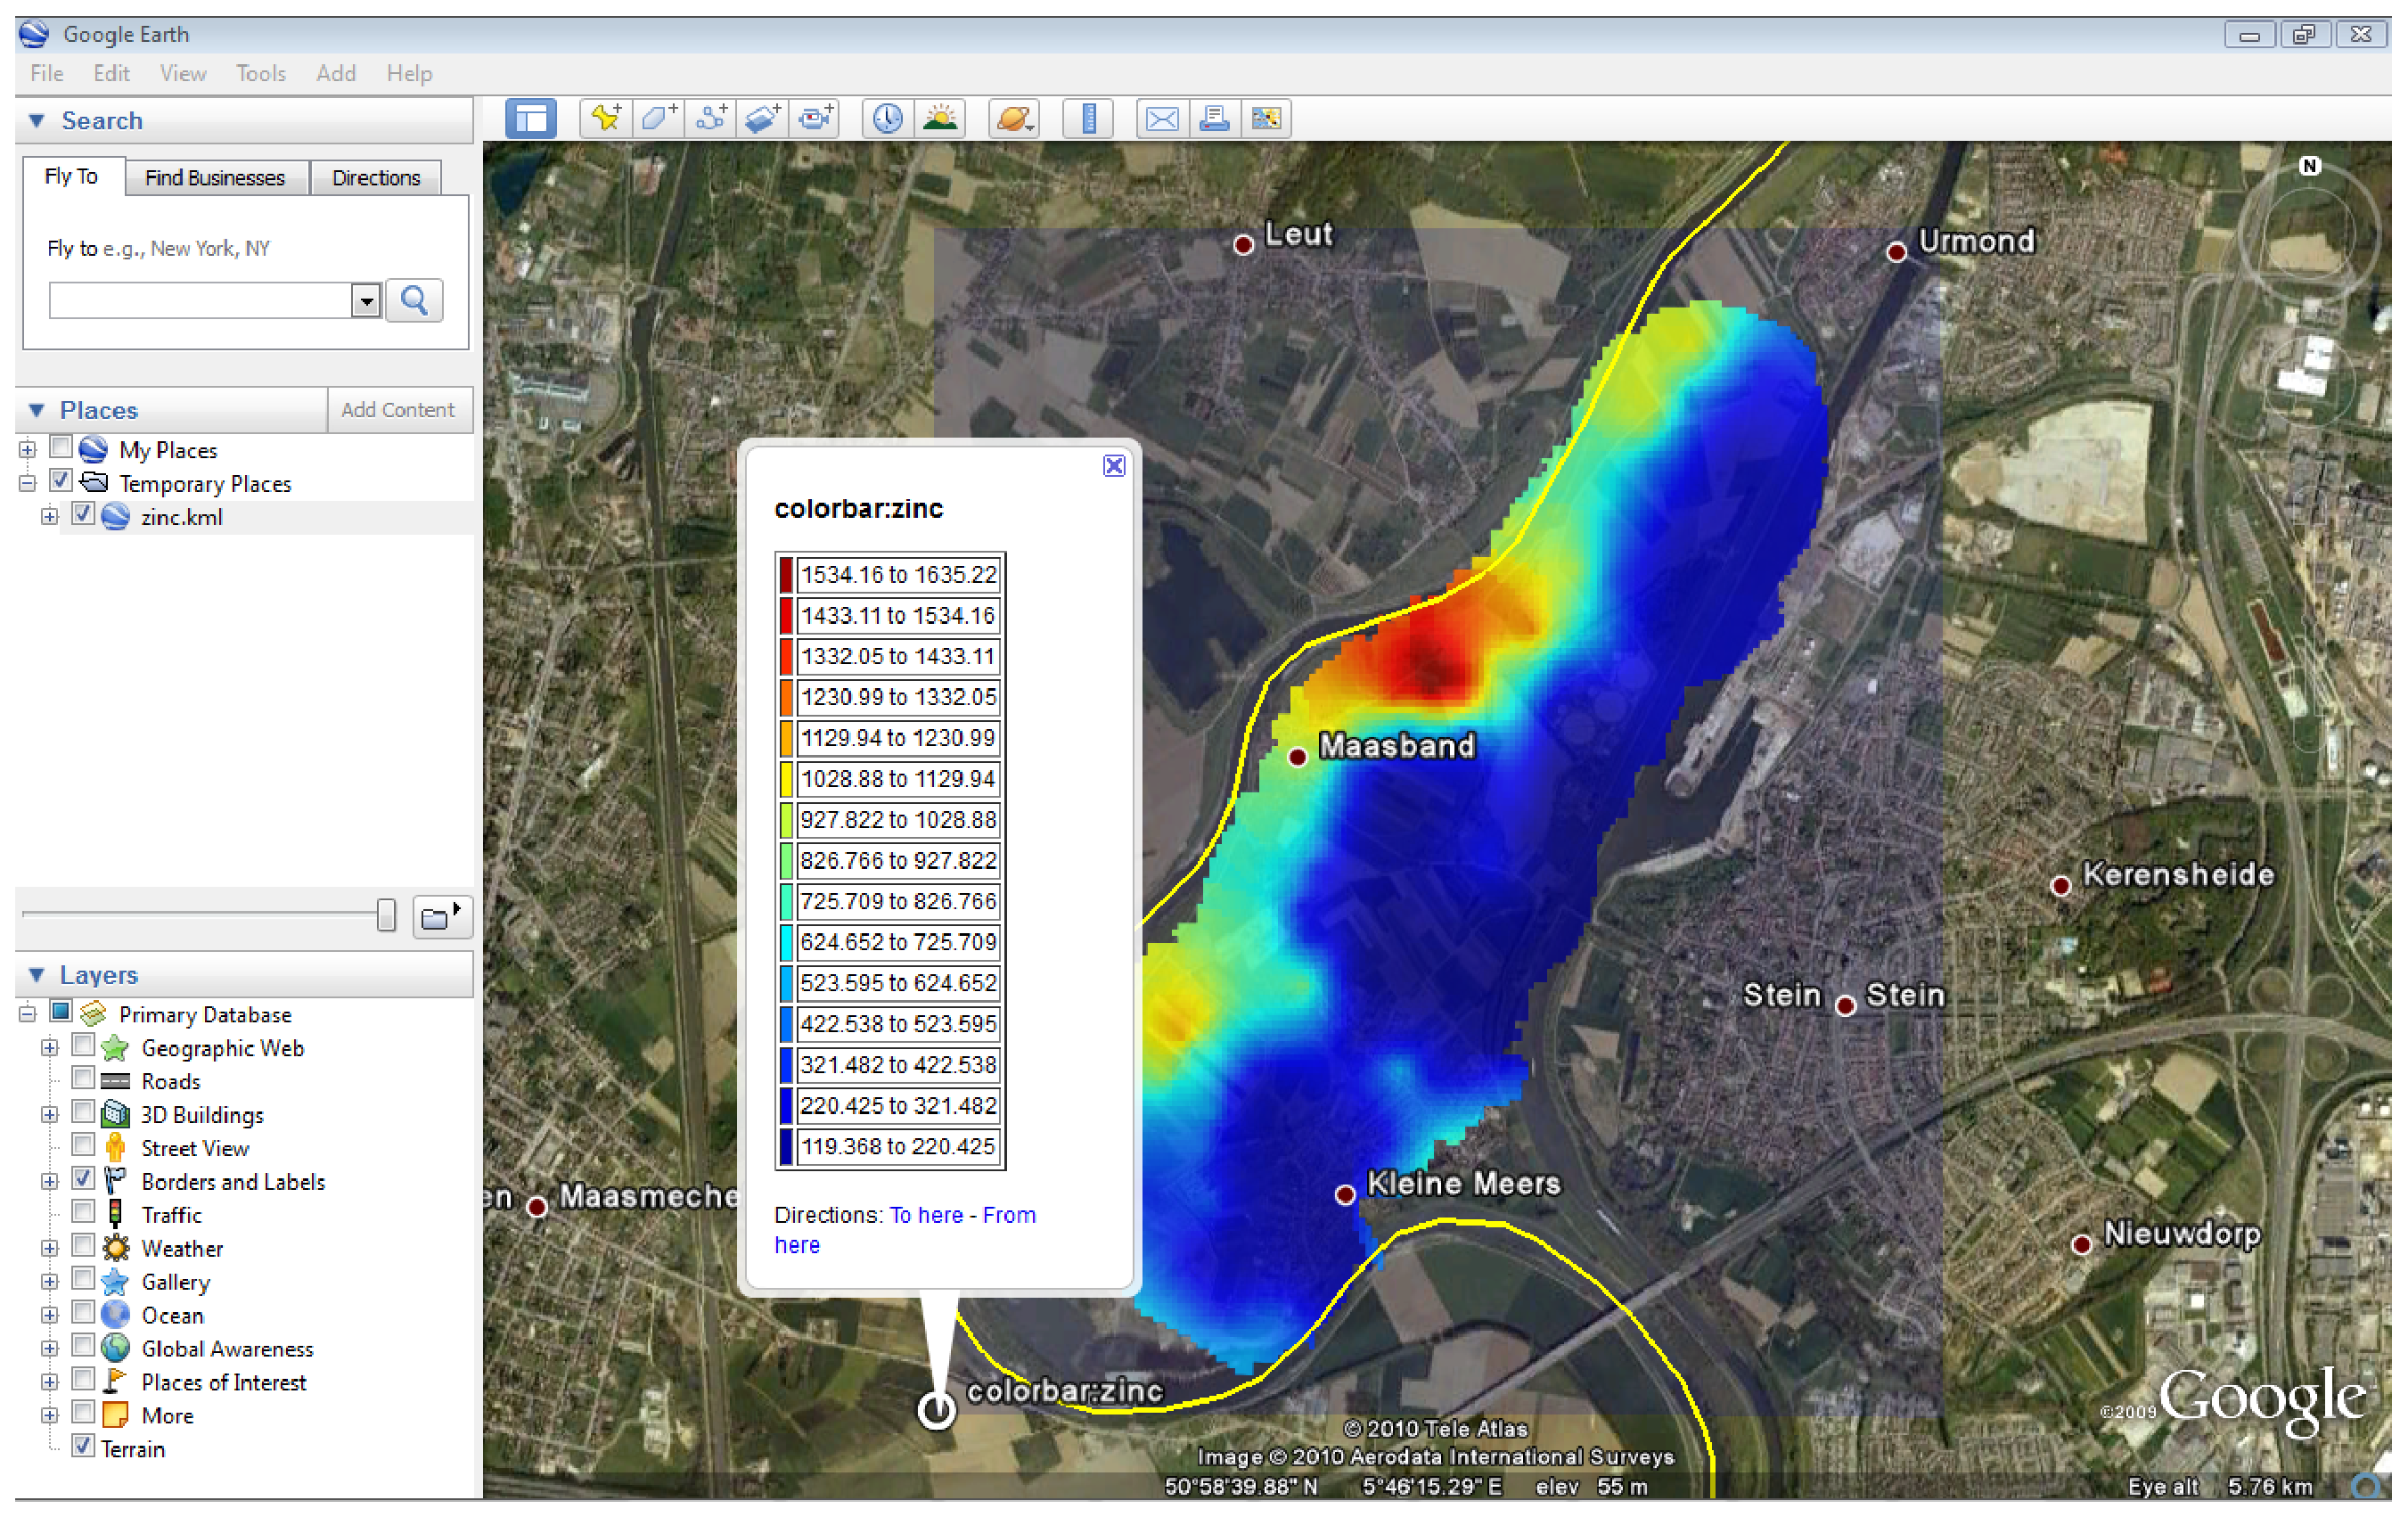
\includegraphics[width=1.0\textwidth]{./../eps/zinc-stein.eps}}
  \caption{Zinc concentrations near Stein}\label{fig:zinc-stein}
\end{figure}



%\section{Advanced features}
%
%\subsection{Time-variant features}
%In addition to displaying static features, the GoogleEarth Viewer can also visualize dynamic content. 
%
%

%\subsection{Filled contour plots}


\projectfooter



